\documentclass[english,11pt]{beamer}

\DeclareMathOperator{\Cov}{Cov}
\DeclareMathOperator{\Var}{Var}
\DeclareMathOperator{\E}{\mathbb{E}}
\DeclareMathOperator{\Proba}{\mathbb{P}}

\newcommand{\Covb}[2]{\ensuremath{\Cov\!\left[#1,#2\right]}}
\newcommand{\Eb}[1]{\ensuremath{\E\!\left[#1\right]}}
\newcommand{\Pb}[1]{\ensuremath{\Proba\!\left[#1\right]}}
\newcommand{\Varb}[1]{\ensuremath{\Var\!\left[#1\right]}}

% norm
\newcommand{\norm}[1]{\| #1 \|}

\newcommand{\indep}{\rotatebox[origin=c]{90}{$\models$}}





\usepackage{mathptmx,amsmath,amssymb,graphicx,bibentry,bbm,babel,ragged2e}

\makeatletter

\newcommand{\noun}[1]{\textsc{#1}}
\newcommand{\jitem}[1]{\item \begin{justify} #1 \end{justify} \vfill{}}
\newcommand{\sframe}[2]{\frame{\frametitle{#1} #2}}

\newenvironment{centercolumns}{\begin{columns}[c]}{\end{columns}}
%\newenvironment{jitem}{\begin{justify}\begin{itemize}}{\end{itemize}\end{justify}}

\usetheme{Warsaw}
\setbeamertemplate{footline}[text line]{}
\setbeamercolor{structure}{fg=purple!50!blue, bg=purple!50!blue}

\setbeamersize{text margin left=15pt,text margin right=15pt}

\setbeamercovered{transparent}


\@ifundefined{showcaptionsetup}{}{%
 \PassOptionsToPackage{caption=false}{subfig}}
\usepackage{subfig}

\usepackage[utf8]{inputenc}
\usepackage[T1]{fontenc}



\makeatother

\begin{document}


\title{Un Cadre de Connaissances pour une G{\'e}ographie Integr{\'e}e}

\author{J.~Raimbault$^{1,2}$\\
\texttt{juste.raimbault@parisgeo.cnrs.fr}
}


\institute{$^{1}$UMR CNRS 8504 G{\'e}ographie-cit{\'e}s\\
$^{2}$UMR-T IFSTTAR 9403 LVMT\\
}


\date{JIG 2017 - Paris\\\smallskip
6 Avril 2017
}

\frame{\maketitle}





%%%%%%%%%%%%%%%%%%%
%% ABSTRACT

% Keywords : Cadre de Connaissances ; Integration des Domaines

% Contexte Les bouleversements techniques et méthodologiques qu’une discipline peut subir sont souvent accompagnés de profondes mutations épistémologiques, voire de la nature même de la discipline. Il est indéniable que les différentes géographies sont actuellement dans cette situation, au regard des nouvelles opportunités en terme de données et de puissance de calcul. Les visions pour des directions futures sont diverses, et peuvent donner par exemple l’emphase sur les données massives (Batty (2012)) ou sur la simulation de modèles par calcul intensif (Pumain and Reuillon (2017a)). Il est crucial de rester conscient des pièges que tend l’usage inconsidéré de ces nouvelles techniques (Raimbault (2016)), et une intégration saine des théories, connaissances, outils, méthodes est une réponse possible.
%Pour une Géographie Intégrée Cette communication se positionne de manière originale en proposant un cadre de connaissances alternatif pour les études ayant une composante quantitative, ou plus préci- sément se posant dans la lignée de la Géographie Théorique et Quantitative (TQG). Ce cadre tente de répondre aux contraintes suivantes : (i) transcender les frontières artificielles entre quantitatif et qualitatif ; (ii) ne pas favoriser de composante particulière parmi les moyens de production de connaissance (aussi divers que l’ensemble des méthodes qualitatives et quantitatives classiques, les méthodes de modélisation, les approches théoriques, les données, les outils), mais bien le développement conjoint de chaque com- posante. Nous étendons le cadre de connaissances de Livet et al. (2010), qui consacre le triptyque des domaines empiriques, conceptuels et de la modélisation, en y ajoutant les domaines à part entière que sont les méthodes, les outils (qu’on peut voir comme des proto-méthodes) et les données. Les interactions entre chaque domaine sont détaillées, comme par exemple le passage des méthodes vers les outils qui consiste en l’implémentation, ou le passage de l’empirique aux méthodes comme prospection méthodologique. Toute démarche de production de connaissance, vue comme une perspective au sens de Giere (2010), est une combinaison complexe des six domaines, les fronts de connaissance dans chacun des domaines étant en co-évolution. Nous nommons notre cadre de connaissance Géographie Intégrée, pour souligner à la fois l’intégration des différents domaines mais aussi des connaissances qualitatives et quantitatives, puisque les deux se fondent dans chacun des domaines : l’empirique peut autant contenir des résultats issus d’analyse de données que d’enquêtes qualitatives de terrain; la modélisation également; la théorie se place à un niveau conceptuel supérieur; les outils et méthodes sont de nature variée et de plus en plus intégrée; et enfin les données sont évidemment de différents types.
%Application L’aventure de l’ERC Geodivercity (Pumain and Reuillon (2017b)) est l’allégorie du cadre proposé. L’intégration de la théorie, de l’empirique, de la modélisation, mais aussi de la technique et de la méthode, n’a jamais été aussi creusée et renforcée que dans les divers développements du projet. Sans
%l’accès à la grille de calcul et aux nouveaux algorithmes d’exploration permis par OpenMole, les connais- sances tirées du modèle SimpopLocal auraient été moindres, mais les développements techniques ont aussi été conduits par la demande thématique. D’autres exemples concrets issus de notre travail de recherche illustrent également le rôle de chacun des domaines, et le besoin d’intégration entre chaque. Un premier exemple étudie les interactions entre réseaux et territoires, du point de vue de la morphologie urbaine et des réseaux. Les corrélations entre indicateurs de forme urbaine et mesures de réseau sont calculées sur l’ensemble de l’Europe. Des outils spécifiques de simplification du réseau routier sont développés pour rendre les traitement faisable en terme de temps de calcul et de mémoire utilisée, et des méthodes liant correlations temporelles et spatiales sont proposées. Les connaissance empiriques tirées de l’intégration des méthodes, outils et données, permettent de formuler des hypothèses théoriques, comme une confirmation à échelle moyenne de la théorie évolutive des villes de par la non-stationnarité spatiale des correlations entre réseaux et forme urbaine. Un autre exemple qui relève de l’épistémologie quantitative, consiste en la reconstruction sous forme d’un réseau sémantique de l’horizon scientifique des travaux traitant des rela- tions entre réseaux et territoires. Les communautés distinctes au sein du réseau confirment la segmentation en domaines ayant peu d’interactions et aux enjeux différents, ce qui pourrait être un facteur explicatif du faible nombre de modèles couplant croissance urbaine et croissance des réseaux. Dans cette étude, les hypothèses théoriques initiales guidées par une revue manuelle de littérature, guident la conception de nouvelles méthodes (hyper-réseau citation et sémantique) et des outils correspondants (collecte de données massives), qui permettent la construction de jeux de données originaux et leur analyse empirique, pour finalement revenir à la théorie.
%Malgré les idées reçues, le quantitatif se prête particulièrement bien à l’alternatif, notamment car il requiert de cadrer les progrès techniques pour pouvoir en tirer des connaissances pertinentes. Le position- nement de notre cadre de connaissances propose une voie alternative vers une intégration des domaines permettant de considérer la production de connaissance au delà des distinctions entre quantitatif et qua- litatif, et possiblement une intégration des disciplines puisque son application n’a pas de raison d’être limitée à la géographie. Nous postulons qu’il pourrait permettre de se rapprocher des objectifs d’intégra- tion horizontale et verticale pour une Science des Systèmes Complexes (Chavalarias et al. (2009)), c’est à dire la production de disciplines intégrées (vu l’importance de l’émergence dans le cadre initial) et l’étude de questions fondamentales transversales.





%%%%%%%%%%%%%%%%%
\section{Introduction}
%%%%%%%%%%%%%%%%%

%%%
% Examples of co-adaptation tools/theory ? 
%  -> find an introducing anecdote
%
%  - expliquer pourquoi on n'enfonce pas des portes ouvertes : exemples de bloquages, réticences etc.

\sframe{Un Alternatif Auto-organisé}{

\justify

\vspace{-0.5cm}

\textit{Les mutations des objets entraînent des mutations épistémologiques : cf. Habitat participatif H. Milet ; l'instrumentalisation des objets est conditionnée aux mutations des positionnement épistémologiques ou politiques : cf. squat artistique J. Pinard.}

\medskip

\textit{De même pour la mutation des techniques et méthodes : différentes réactions possibles au même phénomène, comme l'emphase sur les données massives \cite{batty2012smart} ou sur le calcul intensif \cite{pumain2017book}}

\bigskip

$\rightarrow$ Quelle intégration des différentes composantes de la connaissance ?

\bigskip

\textbf{{\fontencoding{U}\fontfamily{futs}\selectfont\char 66\relax}} Enfoncer des portes ouvertes ? \textit{Si personne n'y rentre sont-elles vraiment ouvertes ? cf. \cite{legavre1996neutralite}}

}





\sframe{Objectif}{

% type "question de recherche"




\textit{Le cadrage épistémologique comme outil pour comprendre et guider l'intégration ?}

\justify

\medskip

\textbf{Cadres existants (exemples dans d'autres disciplines) : } \cite{carlile2004transferring} : sociologie de l'innovation ; \cite{durantin2017disruptive} : entre ingénierie et design ; \cite{gemino2004framework} : évaluation des grammaires dans les systèmes d'information ; \cite{cottineau2015modular} : Cadre de multi-modélisation pour le test d'hypothèses.

\medskip

\textbf{Question de recherche : } \textit{Quel cadre pour rendre compte de la nature complexe des constructions de connaissances, et tirer parti de celle-ci de manière réflexive ?}

}





%%%%%%%%%%%%%%%%%
\section{Cadre de connaissances}
%%%%%%%%%%%%%%%%%


\sframe{Contexte}{

\justify

\textbf{Géographie Théorique et Quantitative : } Un renouvellement de la géographie, plus subtil qu'un simple apport de méthodes mathématiques\\\cite{pumain2002role} ; une exception francophone ? \cite{cuyala2013diffusion}

\bigskip

%(i) transcender les frontières artificielles entre quantitatif et qualitatif
%(ii) ne pas favoriser de composante particulière parmi les moyens de production de connaissance (aussi divers que l’ensemble des méthodes qualitatives et quantitatives classiques, les méthodes de modélisation, les approches théoriques, les données, les outils), mais bien le développement conjoint de chaque com- posante.

\textbf{Contraintes pour le cadre}

\begin{enumerate}
\item Intégration des disciplines (objets géographiques par nature interdisciplinaires)
\item Intégration des domaines de connaissance : pas de composante privilégiée
\item Au delà des frontières artificielles ``quantitatif-qualitatif'' : intégration des méthodes
\end{enumerate}




}




\sframe{Cadre de base}{

% schema Livet Sanders et al. 2010

\textit{Cadre initial proposé par \cite{livet2010} : Interaction et complémentarité des domaines de connaissance}

\bigskip
\bigskip

\centering
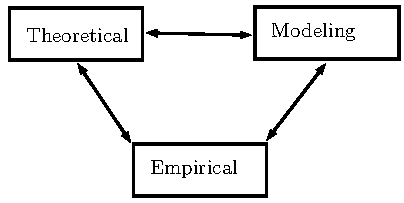
\includegraphics[width=0.7\textwidth]{figures/tqgSimple}



}



\sframe{Fondements Epistémologiques}{

% Perspectivisme de Giere
%   Giere : explaining Science
%   Feyereabend justifying perspectivism ?
% positionnement % Hacking ?

%  // link with formal framework socio-eco systems ? -> in dvlpmt ?

% Pour une épistémologie appliquée ?

\justify

1. Une approche cognitive de la Science~\cite{giere2010explaining} : les \textit{agents} scientifiques~\cite{giere2010agent} à l'origine des dynamiques co-évolutives des connaissances. Cadre épistémologique du perspectivisme~\cite{giere2010scientific}.

\bigskip

2. Compatible avec une \textit{science anarchiste} à la Feyerabend \cite{feyerabend1993against} : auto-organisation et émergence des connaissances


\bigskip

3. Extrême sur la ``check-list'' de Hacking~\cite{hacking1999social} (au delà de Kuhn) :
\footnotesize
\begin{itemize}
\item contingence maximale de par la nature dépendante au chemin du processus complexe de co-évolution des connaissances
\item degré de constructivisme maximal dans la posture perspectiviste
\item stabilité des sciences fortement couplée entre origine interne et externe de par le rôle des agents
\end{itemize}


}




\sframe{Formulation (I)}{

% specification and definitions

% first def co-evol and morphogenesis

\justify

\vspace{-0.5cm}

\textbf{Definition.} La morphogenèse d'un système implique des relations circulaires causales et souvent autonomes entre les niveaux d'émergence\\ (\cite{bedau2002downward}) entre \textit{forme} et \textit{fonction} \cite{antelope2016interdisciplinary}, et exhibe dans ce sens une architecture émergente \cite{doursat2012morphogenetic}.

\bigskip

\textbf{Fait stylisé.} Il existe des processus de production de connaissances scientifiques morphogénétiques, constitués d'ensemble de \textit{perspectives}, et impliquant une co-évolution des vecteurs (agents) et de domaines de connaissance (def. ci-dessous).

\bigskip

\textbf{Postulat.} La TQG en fait majoritairement partie et est en ce sens précurseur d'une \textit{Géographie Intégrée}. [Note : appel aux épistémologues, démonstration systématique à effectuer]





}


\sframe{Formulation (II)}{

\textbf{Définition des domaines.}

\begin{itemize}
\item \textbf{Empirique} Connaissances empiriques sur des cas réels
\item \textbf{Théorique} Construction cognitives plus générales
\item \textbf{Modélisation} \textit{Medium} formalisé de la perspective, ou tout modèle au sens de Varenne \cite{varenne2010simulations}
\item \textbf{Données} Information brute qui a été captée
\item \textbf{Méthodes} Structures génériques de production de connaissances
\item \textbf{Outils} Proto-méthodes et supports des autres domaines
\end{itemize}


\medskip

\textbf{Corolaire.} La distinction entre ``quantitatif'' et ``qualitatif'' est arbitraire et sans intérêt pour la production dans ce cadre, de par la nécessité de l'ensemble de leur composantes dans l'ensemble des domaines.  


}



\sframe{Illustration}{

%\footnotesize\textit{Projection of knowledge space as a complete graph (tentative qualifications for binary relations)}

\footnotesize\textit{Projection de l'espace des connaissances comme graphe complet (qualifications arbitraires pour les relations binaires)}


%\medskip

\centering

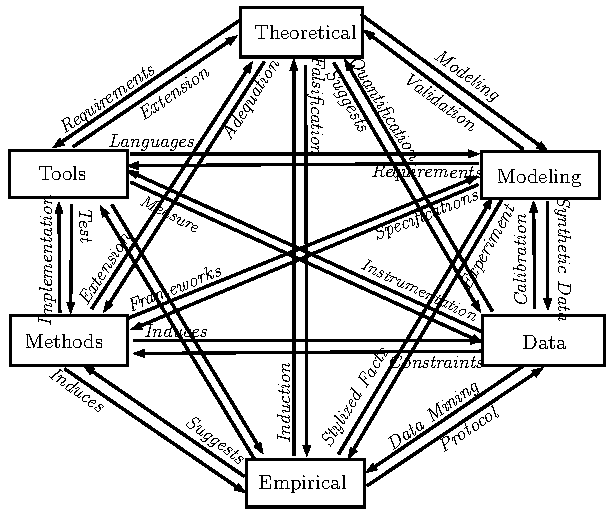
\includegraphics[width=0.7\textwidth]{figures/tqg}

}


\sframe{Implémentation (I)}{

\justify

% meta-modeling, impossibilité d'un cadre unifié, on ne cherche pas à faire du meta-modeling ni à expliquer la production de connaissance en général, mais prendre conscience du processus de co-evolution et de tirer parti de cette prise de conscience.

% sur le meta-modeling, note sur reflexivité-strange loops ?

% \cite{Fanelli04042017} : science ouverte
% ex. ReScience
%  quani-quali : opposer "evidence-based et quali argumenté et contextualisé" (politique InSHS) : pas pertinent.


\vspace{-0.2cm}

\textbf{Implémentation : }Cadre meta, pouvant a priori être traduit dans la plupart des conceptions du modèle

\begin{itemize}
\item Modèles de simulation
\item Modèles statistiques ou mathématiques
\item Modèles de données
\item Modèles conceptuels
\end{itemize}

\bigskip


\textbf{Science Ouverte : } Reproductibilité et transparence \textbf{totales} (sous conditions éthiques) postulées comme nécessaires (positionnement ``politique'' à ce stade, pourrait être étudié systématiquement \cite{Fanelli04042017}). Outils libres et ouverts, collaboratifs etc. (git : cf. \cite{rescience} Journal of Replicated Science)







}

\sframe{Implémentation (II)}{

\textbf{{\fontencoding{U}\fontfamily{futs}\selectfont\char 66\relax} Pièges classiques (exemples) : \textit{aucun des domaines ne s'improvise}}

\bigskip

\begin{itemize}
\item \justify Usage aveugle, non informé ou faux de méthodes et outils (simulation de modèles résolus, complexité d'execution inutile, camouflage de lacunes méthodologiques)
\end{itemize}
\begin{itemize}
\item \justify Etude quantitatives poussées déconnectées de toute théorie : réinvention de l'eau chaude, arrogance disciplinaire~\cite{dupuy2015sciences}
\end{itemize}
\begin{itemize}
\item \justify Usage inconsidéré des données non-conventionnelles \cite{raimbault2016cautious}
\cite{2017arXiv170400480G}
\end{itemize}

}




%%%%%%%%%%%%%%%%%
\section{Discussion}
%%%%%%%%%%%%%%%%%


\sframe{Application : Théorie évolutive des villes}{

\justify

% Application : 
% Lecture de la théorie évolutive au regard de ce fwk (différent application concrète)

% broad view of the importance of knowledge co-evolution in evolutive urban theory
% try to give a sketch of what is it ?

% org des villes dans territoires
%ambition : rassembler essentiel faits stylisés, les placer pas dasn une th disciplinaire, ou equilibre, structure statiques, mais perspectives spatio temporels qui permet de les suivre sur longues periodes de temps ; attention aux principaux facteurs structurants : systèmes ; attention à observer bifurcation ; en ce sens, systèmes complexes pour aider : villes dans des systèmes de ville, Berry considérablement revisité ; ville objet complexe pas indépendant, inséré dans ses réseaux ; mieux 

\vspace{-0.5cm}

{\footnotesize
\textbf{Définition : }\textit{Une Théorie Géographique ayant pour ambition de rassembler la plupart des faits stylisés connus sur les villes et leur organisation dans les territoires, dans une perspective hors-équilibre et non statique, en les suivant sur de longues périodes de temps et mettant une emphase sur les facteurs structurants et les bifurcations.} [Source : Entretien avec D. Pumain, 31/03/2017]
}

\bigskip

$\rightarrow$ Une interaction forte entre chaque domaine dès les travaux précurseurs : manifeste théorique \cite{pumain1997pour} et modélisation \cite{sanders1997simpop} 

\bigskip

$\rightarrow$ De 2010 à 2016, l'ERC Geodivercity a poussé les limites de l'intégration toujours plus loin : relations ``gagnant-gagnant'' avec les informaticiens (OpenMole \cite{reuillon2013openmole} et Meta-heuristiques \cite{10.1371/journal.pone.0138212}), terrains variés et poussés (\cite{swerts2013systemes} \cite{baffi:tel-01389347}), modélisations intégrées (\cite{cottineau2014evolution} \cite{schmitt2014modelisation}), épistémologie 
\\\cite{rey2015plateforme}

}


\sframe{Application : Relations entre Réseaux et Territoires}{

\vspace{-0.4cm}
{\footnotesize \justify
\textit{(Gauche)} : \cite{raimbault2016cautious} Données, outils et méthodes montrant la non-stationnarité spatiale des correlations entre forme urbaine et topologie des réseaux ; \textit{(Centre)} : \cite{raimbault2016generation} modélisation avec couplage simple montre un vaste espace faisable des correlations simulées ; \textit{(Droite)} Multi-modélisation de la co-évolution : vers une Théorie des Systèmes Territoriaux Co-évolutifs en Réseau~\cite{raimbault2016towards}

}

\begin{columns}
\column{0.38\textwidth}
\centering
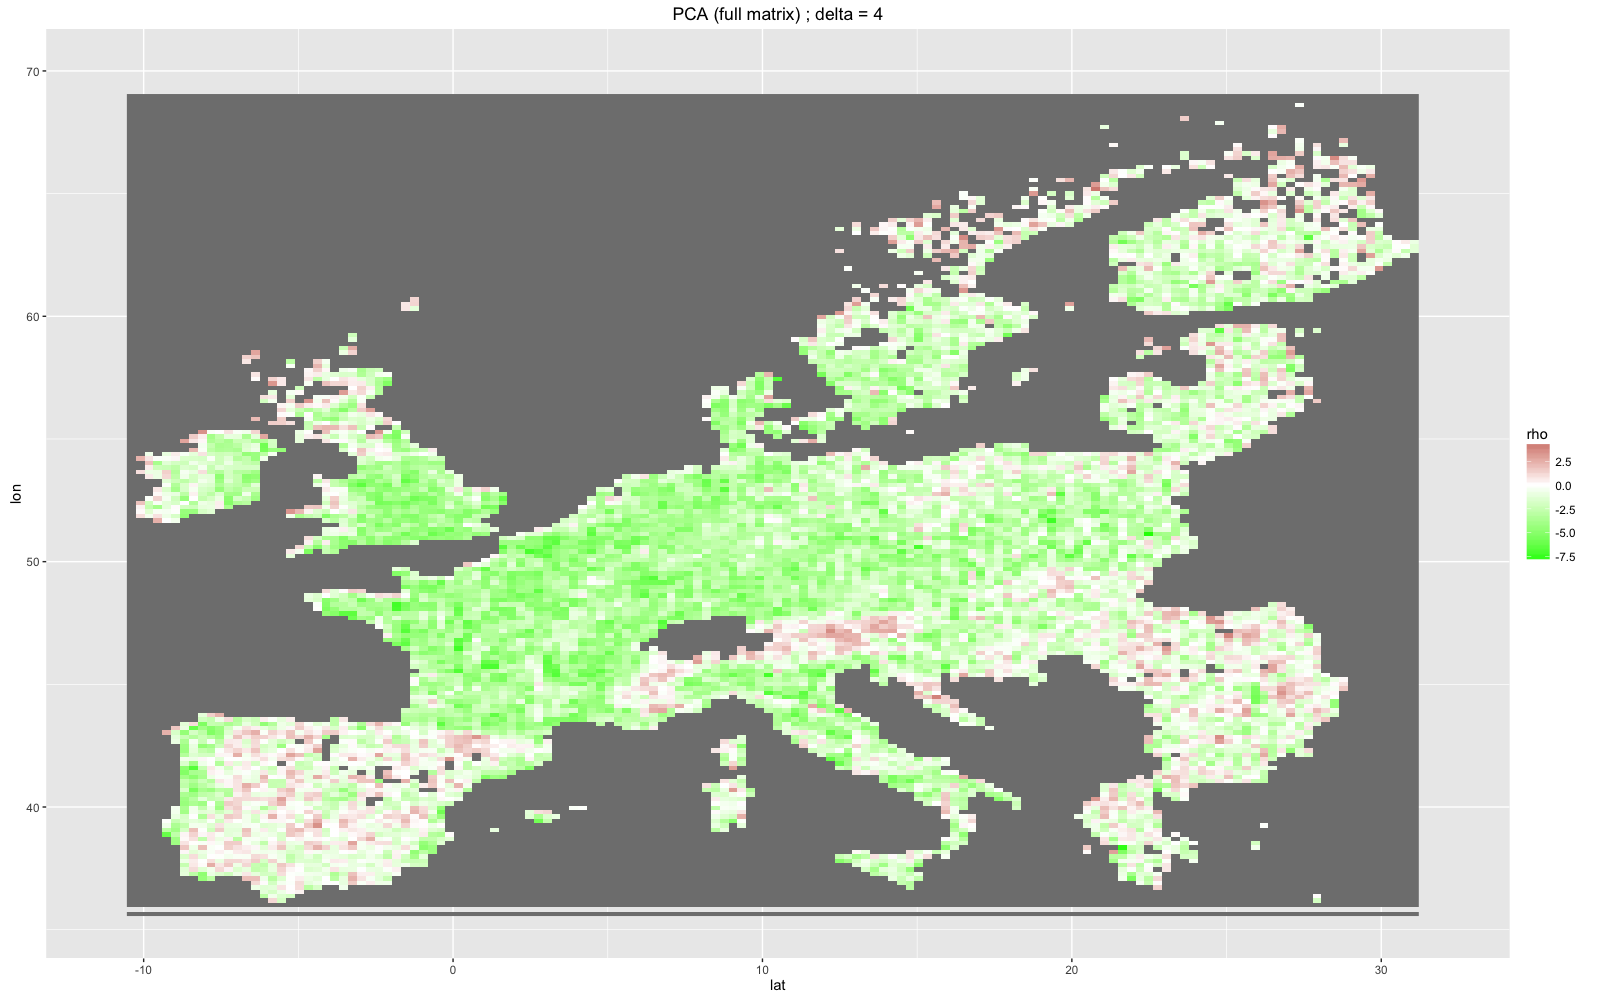
\includegraphics[width=\textwidth]{figures/corr_corr_PCA_delta4}\\
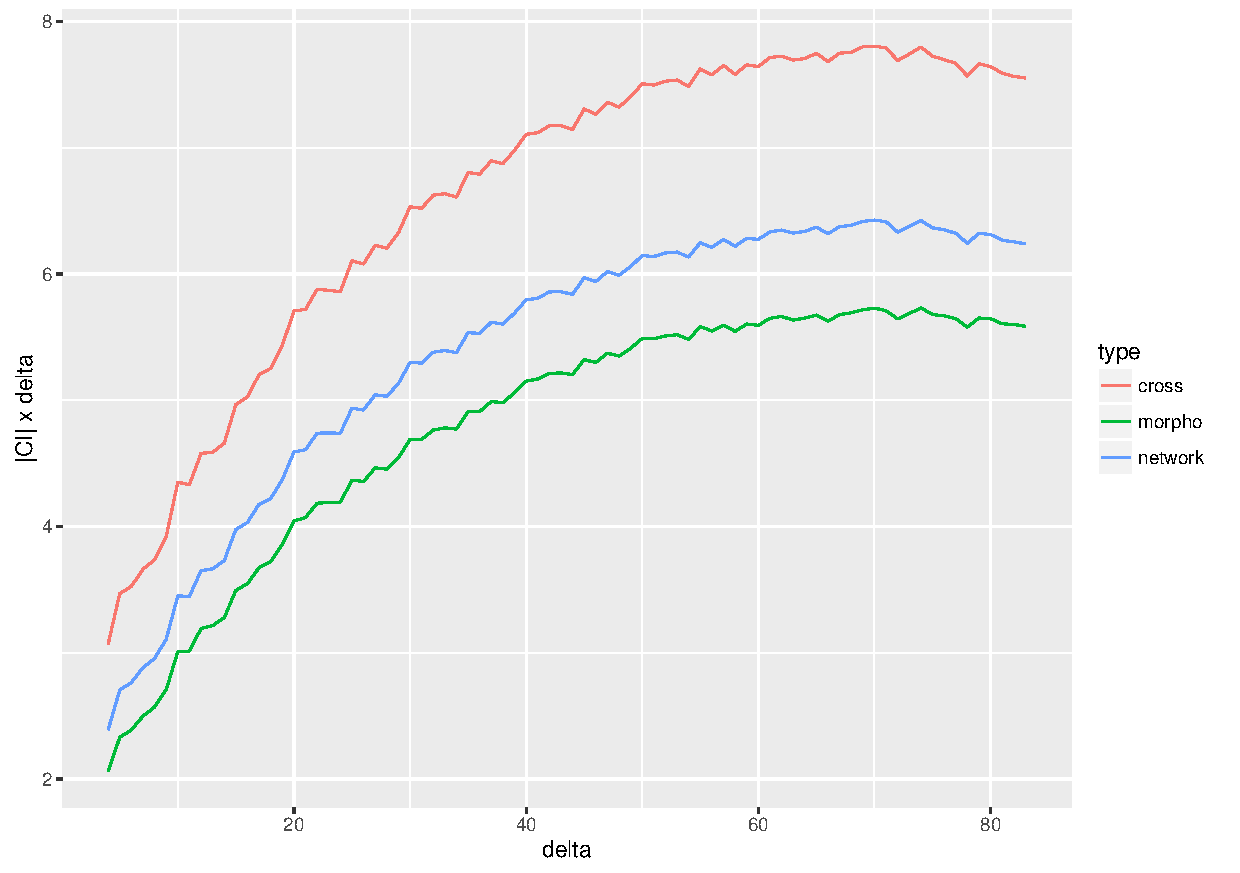
\includegraphics[width=\textwidth]{figures/corr_normalized_CI_delta}

\column{0.22\textwidth}
\centering
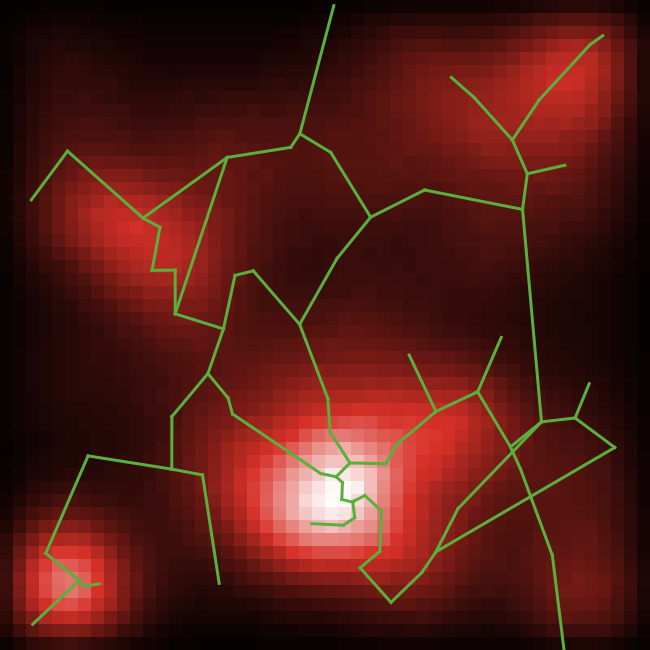
\includegraphics[width=\textwidth]{figures/corr_2_param71913_seed10}\hspace{0.1cm}\\
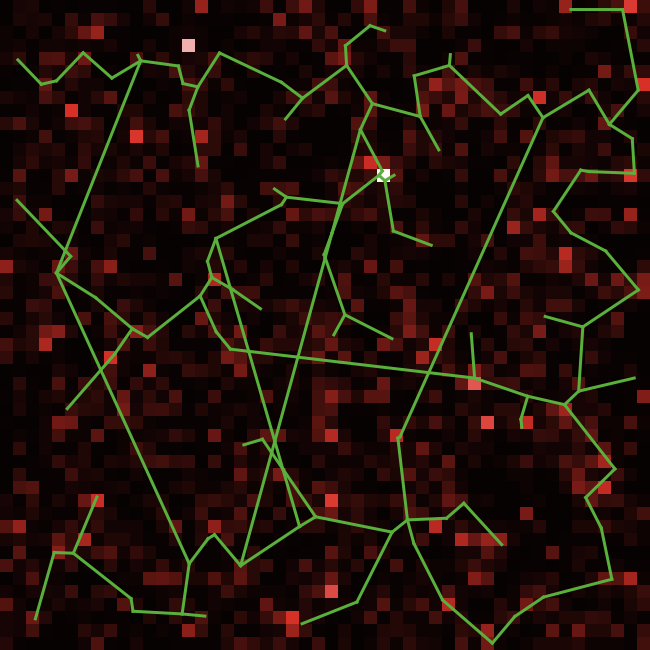
\includegraphics[width=\textwidth]{figures/corr_3_param71918_seed0}

\column{0.22\textwidth}
\centering
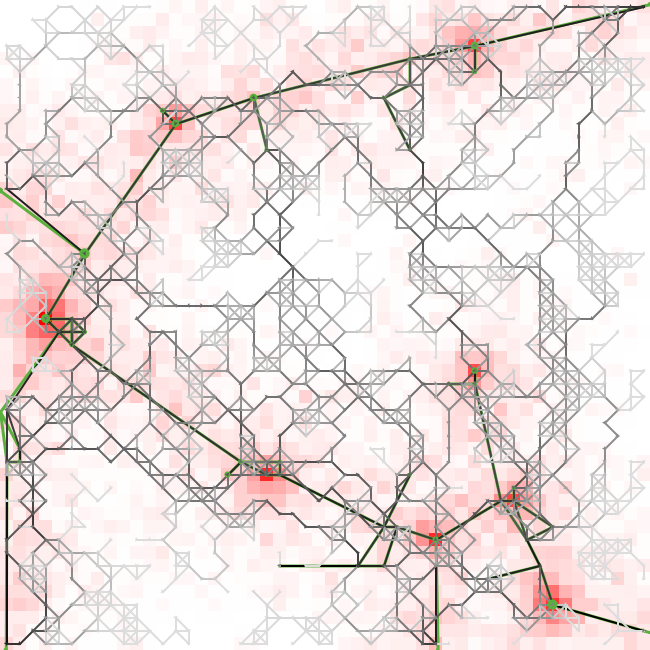
\includegraphics[width=\textwidth]{figures/corr_example-bio-process-0}\hspace{0.1cm}\\
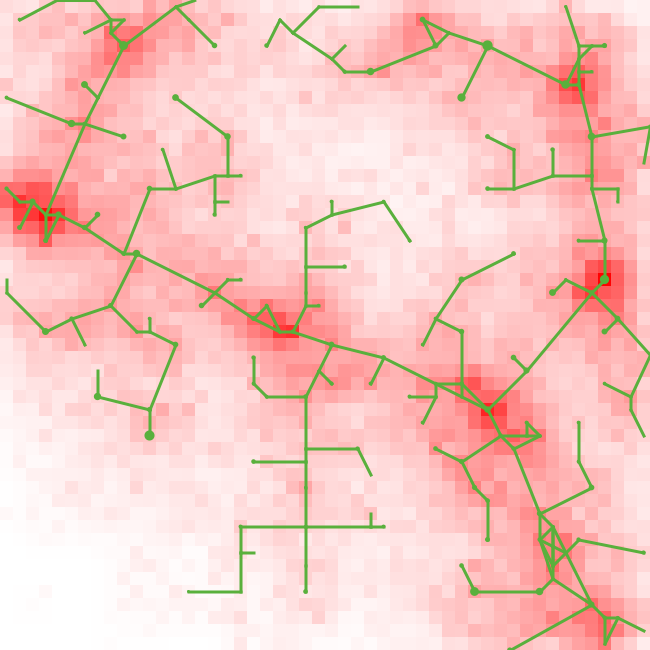
\includegraphics[width=\textwidth]{figures/corr_example-heuristic-0}




\end{columns}
}

\sframe{Application : Epistémologie Quantitative}{

\vspace{-0.4cm}
{\footnotesize \justify
\cite{raimbault2015models} : Revue Systématique Algorithmique reconstruisant la structure sémantique des disciplines étudiant un sujet donné ; Extension des méthodes et outils à une approche par hyperréseau dans \cite{raimbault2016indirect} ; Application à un corpus d'un autre type (brevets) \cite{bergeaud2017classifying} : nouvelle façon d'étudier empiriquement la diffusion spatiale des innovations ? (validation de la Théorie Evolutive urbaine)

}
\medskip

\centering
\includegraphics[width=0.48\textwidth]{figures/cyb_semantic}\hspace{0.2cm}
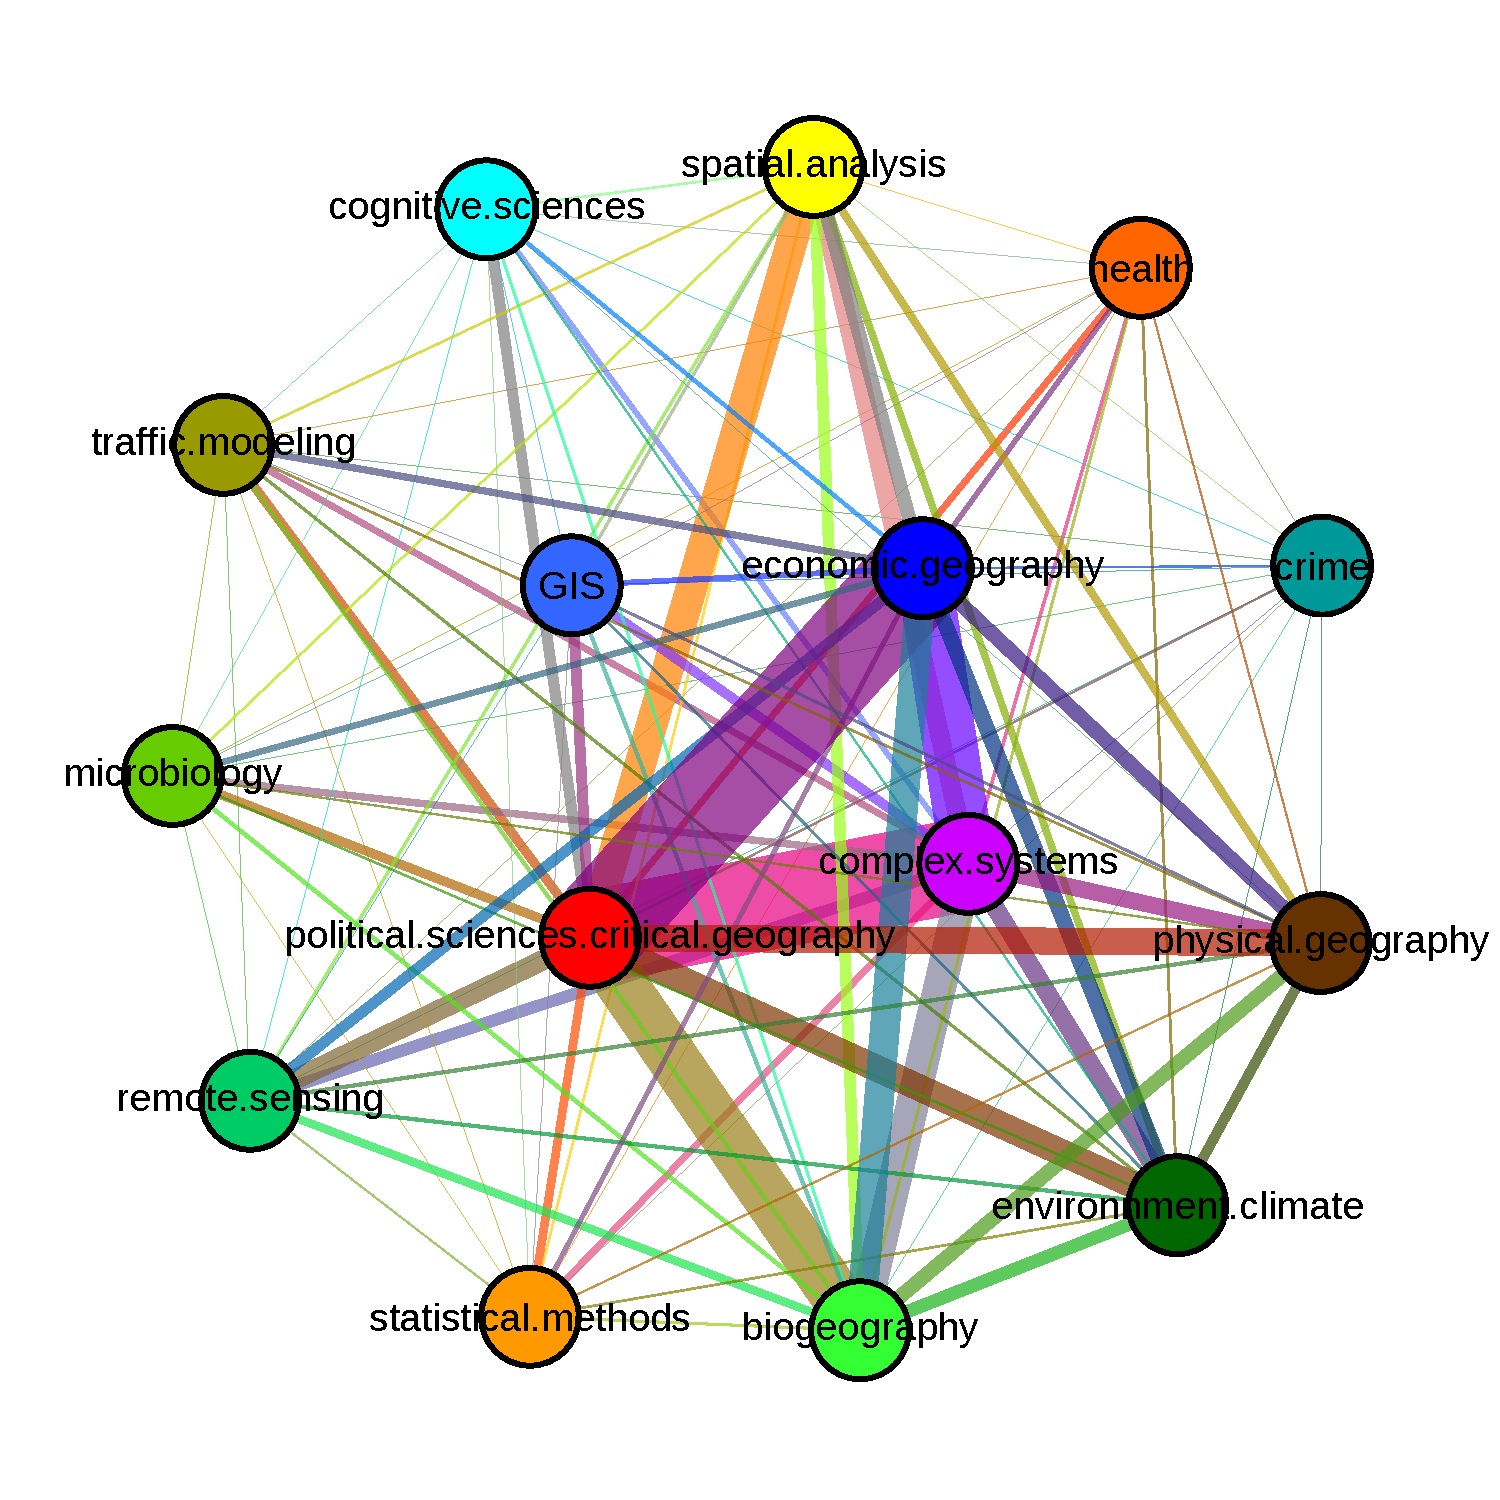
\includegraphics[width=0.48\textwidth]{figures/cyb_synththemcyb}

}


\sframe{Application : Modélisation des Dynamiques Migratoires}{

\textit{Modélisation intégrée des dynamiques migratoires dans le Delta de la Rivière des Perles \cite{losavio2017modeling}}

\bigskip
\bigskip

\centering
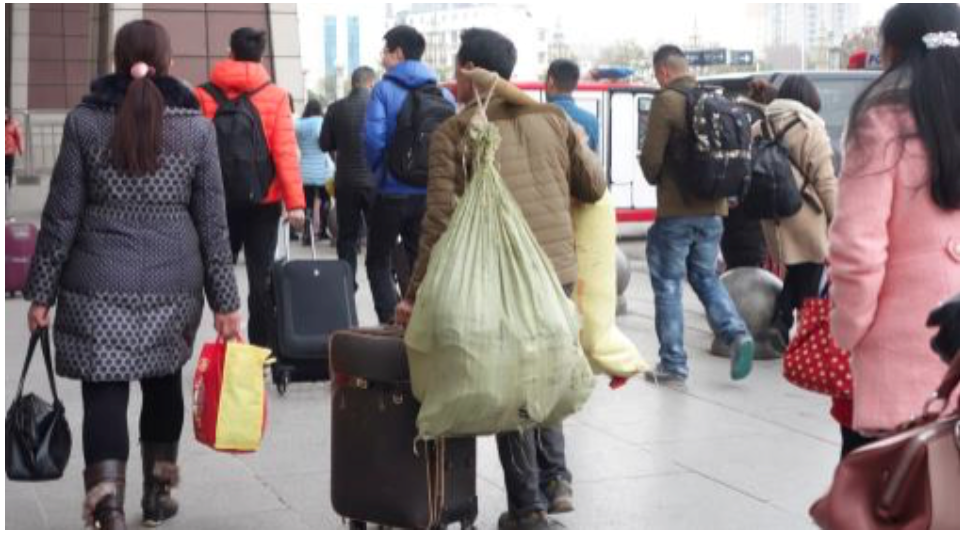
\includegraphics[width=0.48\textwidth]{figures/migration_migrants}\hspace{0.2cm}
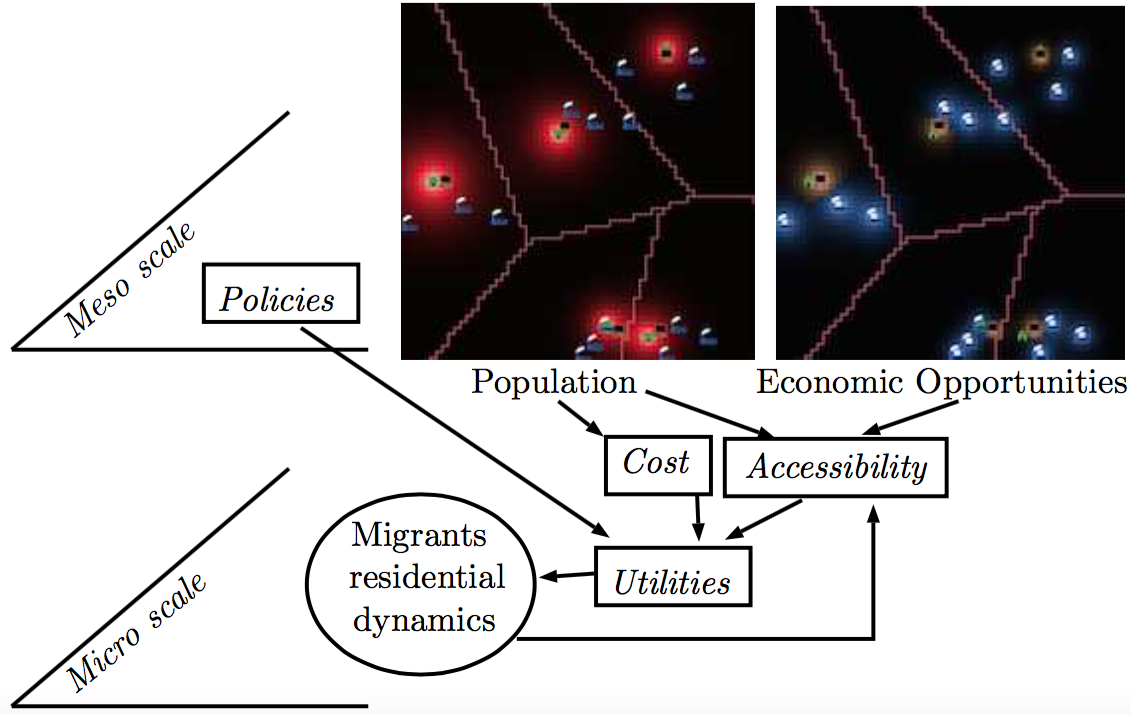
\includegraphics[width=0.48\textwidth]{figures/migration_model}

}






\sframe{Discussion}{

\justify

% Vers un integration horizontale et verticale ? ; cf roadmap. y ajouter la "profondeur" ? (quanti-quali : méthodes ?)

\vspace{-0.4cm}

\textbf{Extension Possible : } \textit{Lien avec un Cadre Formel pour la Modélisation des Systèmes Socio-techniques. Perspectives comme Dataflow Machines \cite{golden2012modeling} munis d'une ontologie \cite{livet2010}, définition de relations d'ordre entre ontologies via émergence \cite{bedau2002downward}, réduction en une forêt ontologique minimale, action de monoïde sur les données.}

\bigskip

\textbf{Perspective : } \textit{Cadre comme un moyen de favoriser l'intégration horizontale (interdisciplinarité et questions transversales) et verticale (disciplines intégrée) de la feuille de route des Systèmes Complexes, en y ajoutant une dimension des domaines de connaissance ? \cite{2009arXiv0907.2221B}}


}




\sframe{Conclusion}{

$\rightarrow$ Ni de la méta-modélisation ni une tentative d'explication de la production de connaissances, mais une affirmation de la structure en domaine et co-évolutive de celle-ci, pour la revendiquer et en tirer parti

\medskip

$\rightarrow$ Pas d'éléments spécifiques pour ``lier quanti-quali'' mais un cadre affirmant le caractère nécessaire de l'intégration

\medskip

$\rightarrow$ Une Géographie Intégrée, alternative au ``mainstream'', mais pas si alternative à l'existant car pratiquée depuis une trentaine d'années !



\bigskip
\bigskip
\bigskip


\footnotesize{ - Code et données des différentes études mentionnées disponible sur github à \texttt{https://github.com/JusteRaimbault}
}

}




\sframe{Reserve slides}{

\centering

\Large

\textbf{Reserve Slides}

}




%%%%%%%%%%%%%%%%%%%%%%%%%%%%
\sframe{Theory : Pillars}{
\begin{enumerate}
\item \textit{Networked Human Territories} $\rightarrow$ Raffestin approach to territory combined with Dupuy theory of networks.
\item \textit{Evolutive Urban Theory} $\rightarrow$ City Systems as complex Adaptive systems, applied to human settlements in general and thus territorial systems.
\item \textit{Urban Morphogenesis} $\rightarrow$ Morphogenesis as autonomous rules to explain growth of urban form. Used as the provider of modular decompositions.
\item \textit{Boundaries and Co-evolution} $\rightarrow$ Co-evolution as the existence of \textit{niche}, consequence of boundary patterns.
\end{enumerate}
}
%%%%%%%%%%%%%%%%%%%%%%%%%%%%



%%%%%%%%%%%%%%%%%%%%%%%%%%%%
\sframe{Theory : Specification}{

\textbf{Definition : } Territorial systems are networked Human Territories. They are multi-level complex adaptive systems following Evolutive Urban Theory.

\bigskip
\bigskip
\bigskip


\textbf{Hypothesis : } The existence of Morphogenetic processes in which networks are essential drivers is equivalent to the existence of co-evolutive niches in territorial systems. We call thus these \emph{Co-evolutive Networked Territorial Systems}.

}
%%%%%%%%%%%%%%%%%%%%%%%%%%%%



\sframe{Meso-scale Coupled Growth}{

% RBD model : reproduces some typical urban forms

Simple co-evolutionary dynamics produce stylized urban forms at a mesoscopic scale~\cite{raimbault2014hybrid}

\bigskip
\bigskip

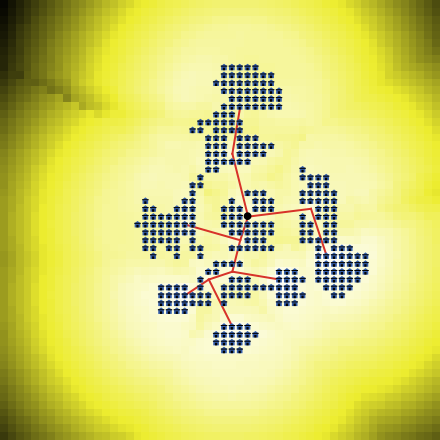
\includegraphics[width=0.3\textwidth]{figures/RBD_lattice}
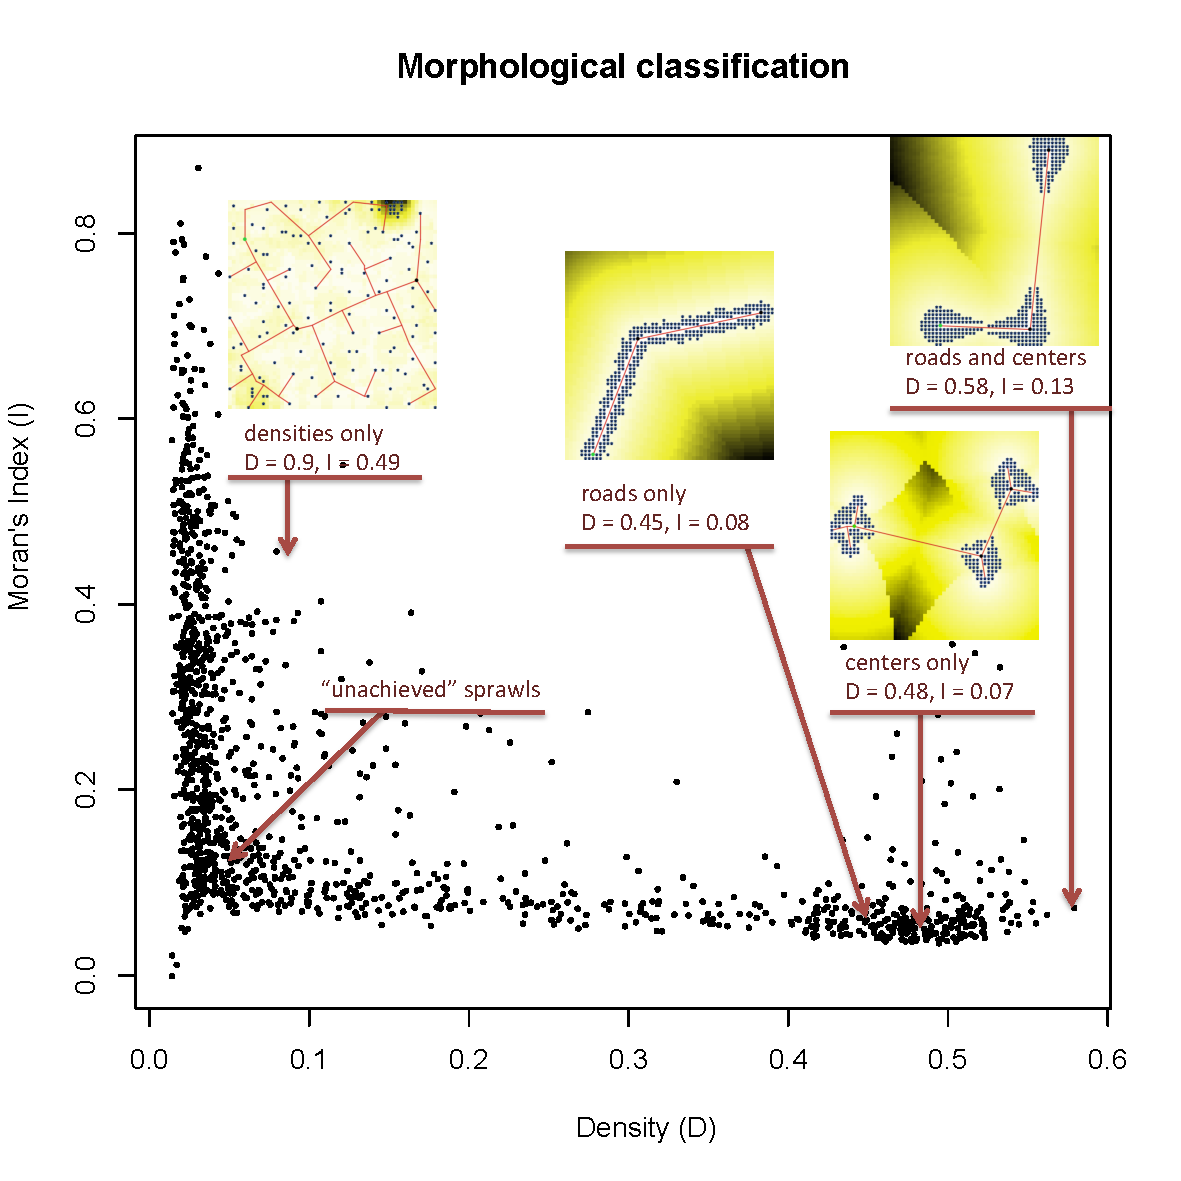
\includegraphics[width=0.35\textwidth]{figures/RBD_morpho}
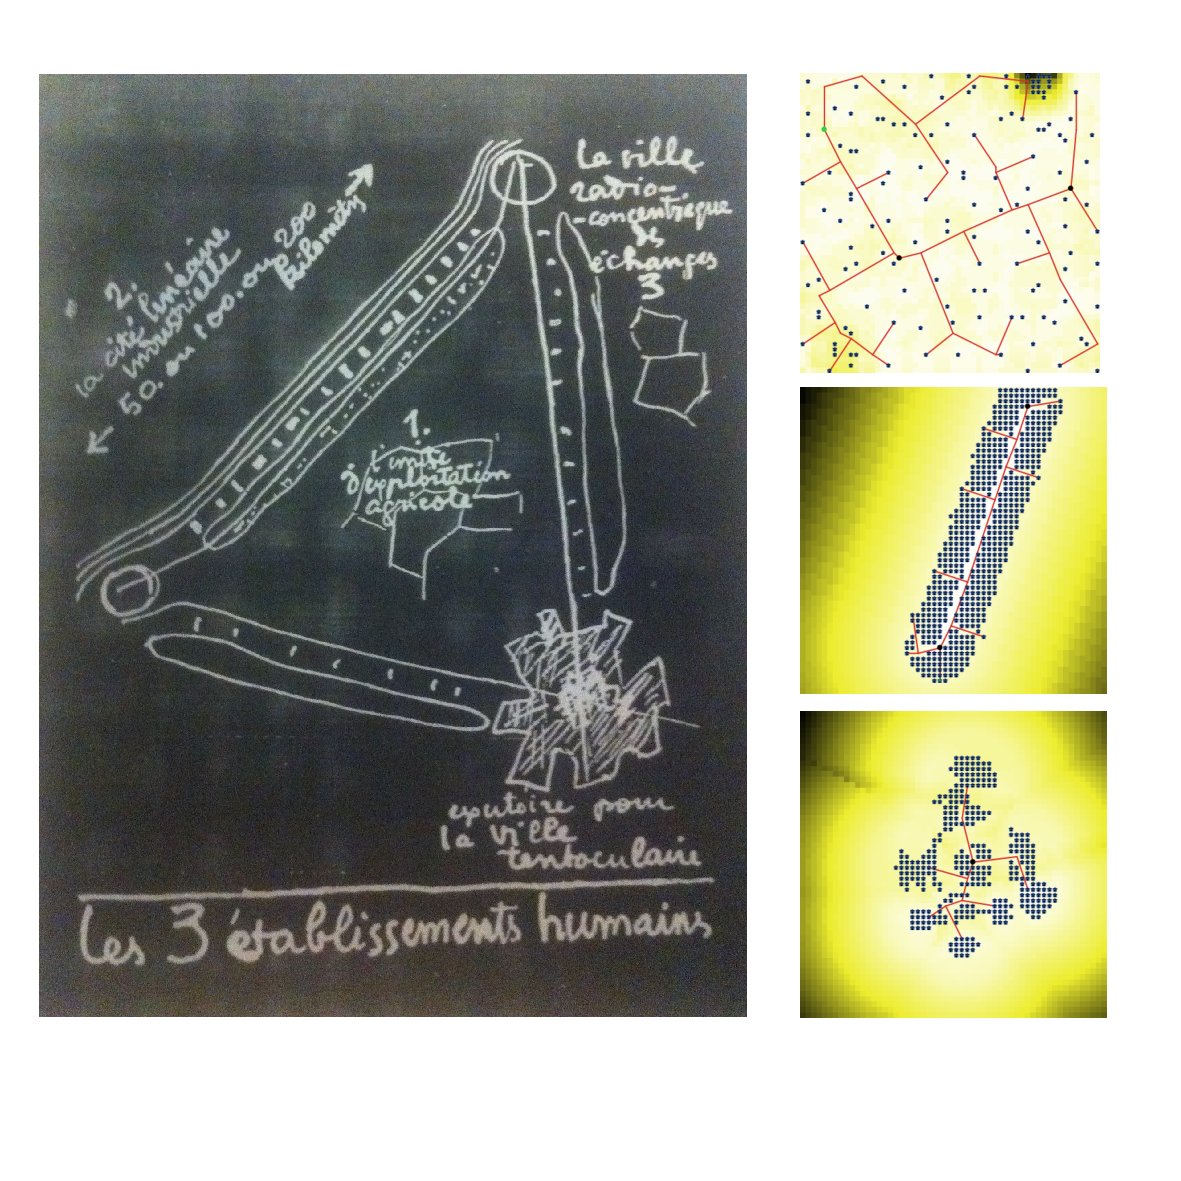
\includegraphics[width=0.35\textwidth]{figures/RBD_corbu}



}



\sframe{Macro-scale Growth and Network Necessity}{


Macro-scale population growth model reveals physical network effects in French System of Cities~\cite{raimbault2016system}


\bigskip

\centering

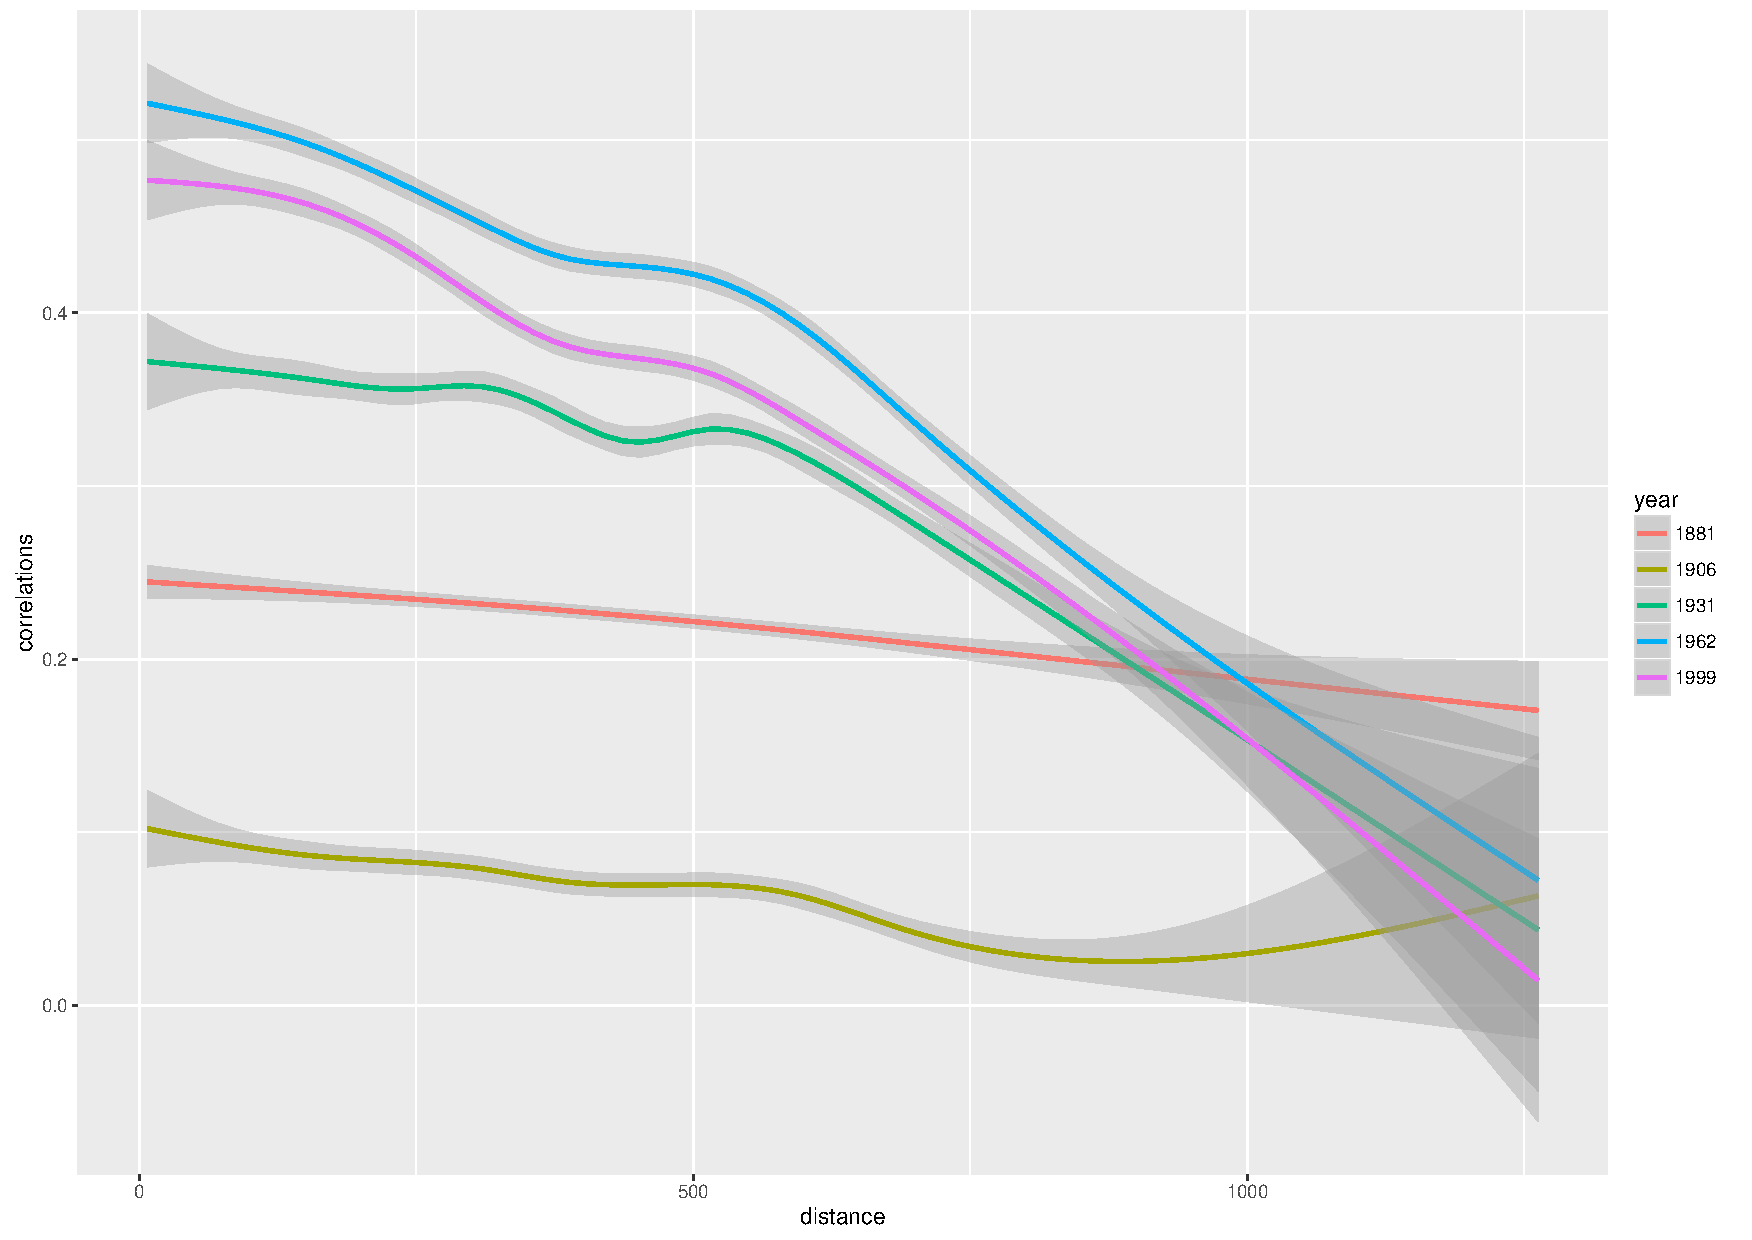
\includegraphics[width=0.3\textwidth]{figures/macro_empirical_tsCorrelations}
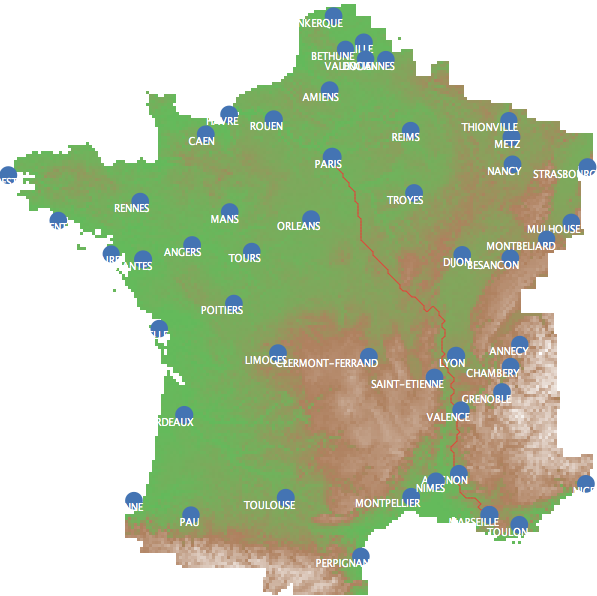
\includegraphics[width=0.3\textwidth]{figures/macro_example_shortest_path}
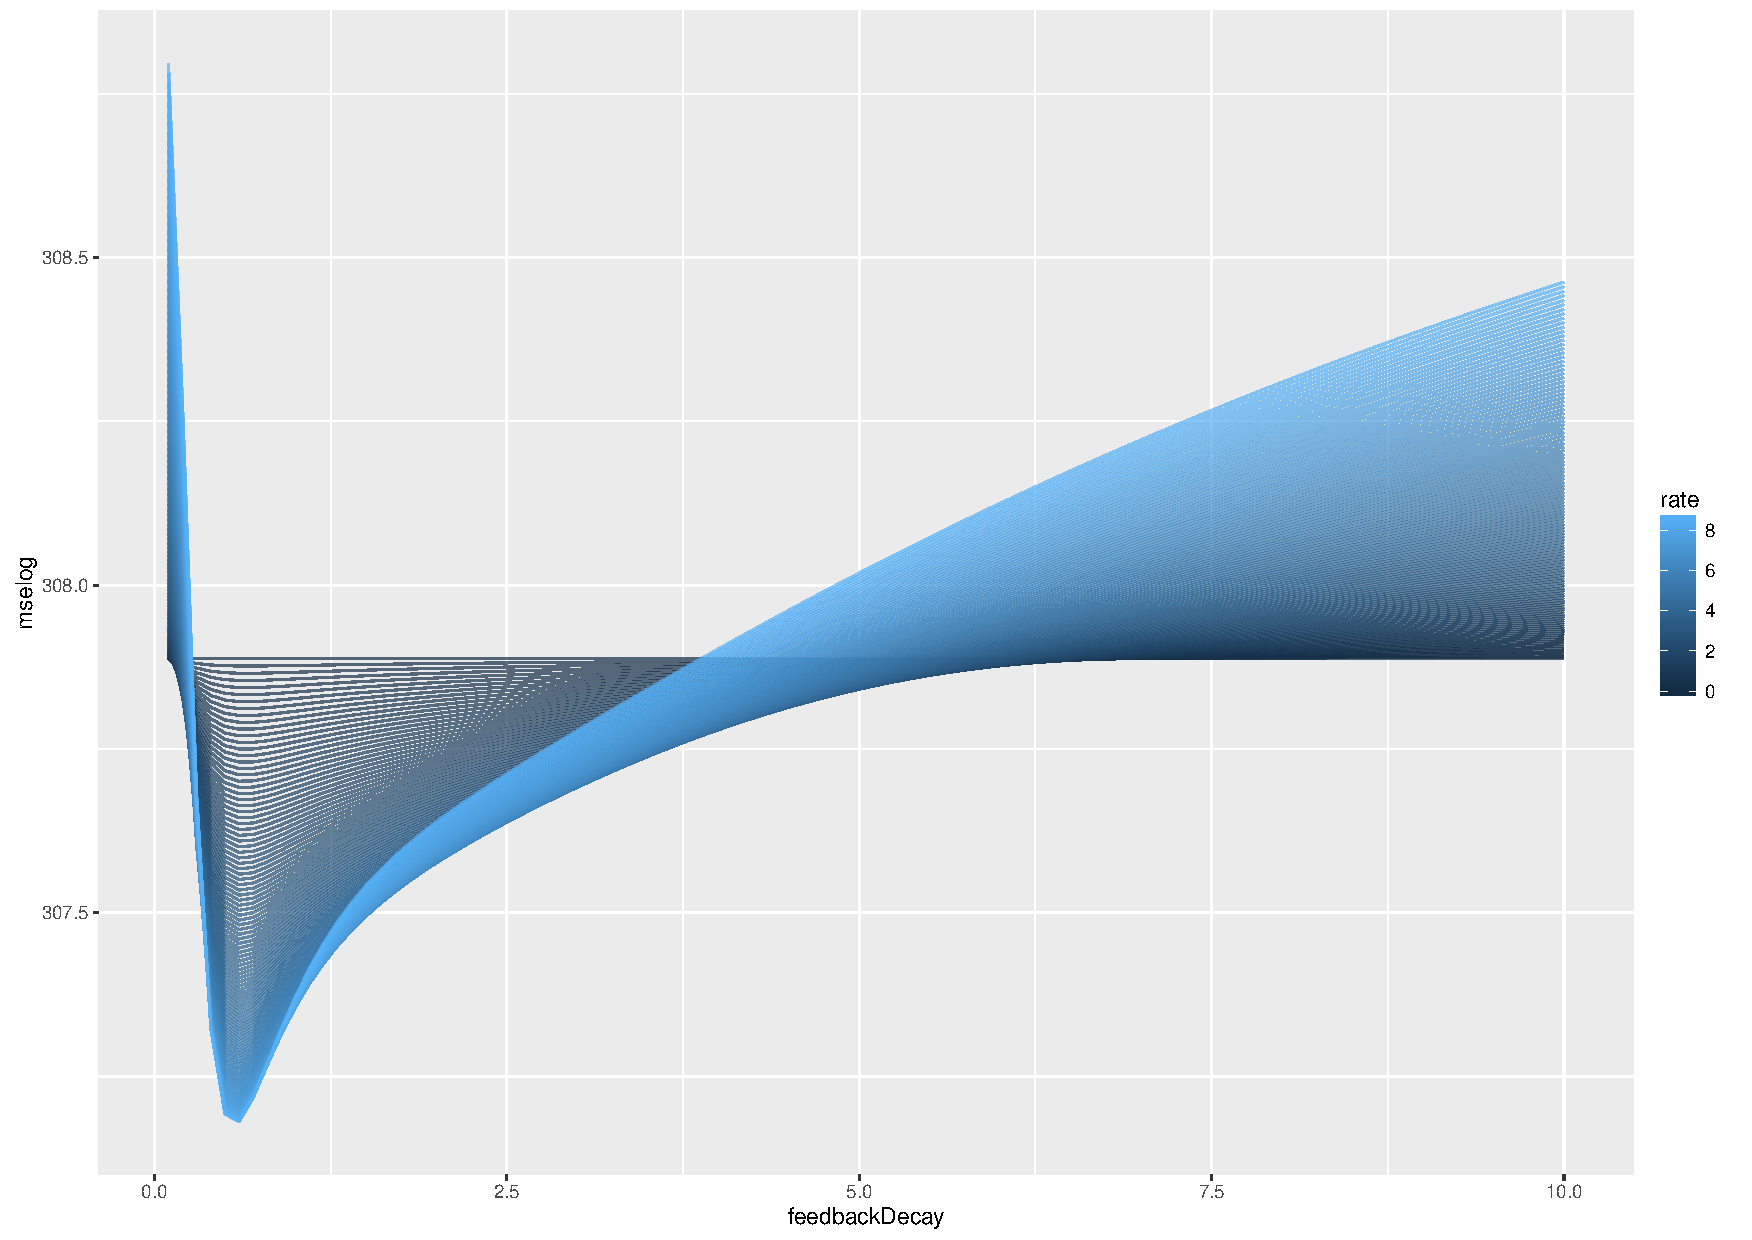
\includegraphics[width=0.3\textwidth]{figures/macro_mselog-feedbackDecay_ZOOM_fixedgravity}

}



\sframe{Extended Formalized Framework: Requirements}{

\begin{itemize}
\item a precise definition and emphasis on the notion of coupling between subsystems, in particular allowing to qualify or quantify a certain degree of coupling : dependence, interdependence, etc. between components.
\item a precise definition of scale
\item a precise definition of what is a system.
\item the notion of emergence in order to capture multi-scale aspects of systems.
\item a central place of ontology in the definition of systems, i.e. of the sense in the real world given to its objects
\item heterogeneous aspects of the same system, that could be heterogeneous components but also complementary intersecting views.
\end{itemize}

}


\sframe{Extended Formalized Framework: Summary}{
$\rightarrow$ Starting from a perspectivist approach to science~\cite{giere2010scientific}, a system is the superposition of perspectives on it, that are dataflow machines~\cite{golden2012modeling} with ontologies~\cite{livet2010}.

\medskip

$\rightarrow$ Compatible notions of \emph{emergence}, nominal and weak emergence~\cite{bedau2002downward}, yield pre-order relations on ontologies.

\medskip

$\rightarrow$ An ontological graph is constructed by induction.

\medskip

$\rightarrow$ The graph can be mapped to a minimal tree (directed forest), that captures a hierarchical structure of the system regarding emergence. ``Strongly coupled'' subsystems are encoded within nodes of the tree.

}










%%%%%%%%%%%%%%%%%%%%%
\begin{frame}[allowframebreaks]
\frametitle{References}
\bibliographystyle{apalike}
\bibliography{/Users/Juste/Documents/ComplexSystems/CityNetwork/Biblio/Bibtex/CityNetwork,biblio}
\end{frame}
%%%%%%%%%%%%%%%%%%%%%%%%%%%%









\end{document}







